% 2010 年江西卷文科第 11 题：正方体 ABCD-A1B1C1D1 与棱 DD1 的中点 M。
% 来源 PDF：普通高考/2010/2010江西文.pdf，SHA-256 c8c86a7272df02211069e27098dcaf04a5cd8af9a9b4d54ffd14a8eb91347af3。
% 原页：第 1 页（A3 三栏）第 2 栏上部，书页码 609。
% 重绘依据：上底 ABCD、下底 A1B1C1D1；M 为棱 DD1 的中点；A1D1、D1C1、DD1 为不可见棱，画虚线。
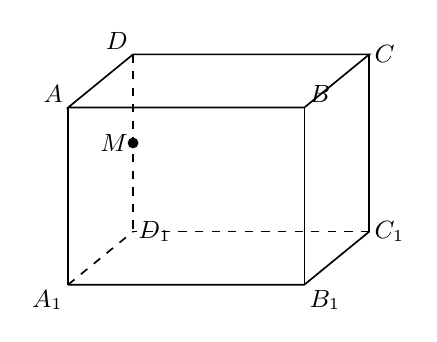
\begin{tikzpicture}[semithick, scale=1.5, every node/.style={inner sep=1.6pt, font=\small}]
  \coordinate (A) at (0,0);
  \coordinate (B) at (2,0);
  \coordinate (C) at (2.55,0.45);
  \coordinate (D) at (0.55,0.45);
  \coordinate (A1) at (0,-1.5);
  \coordinate (B1) at (2,-1.5);
  \coordinate (C1) at (2.55,-1.05);
  \coordinate (D1) at (0.55,-1.05);
  \coordinate (M) at (0.55,-0.3);

  \draw (A) -- (B) -- (C) -- (D) -- cycle;
  \draw (A) -- (A1);
  \draw (B) -- (B1);
  \draw (C) -- (C1);
  \draw (A1) -- (B1) -- (C1);
  \draw[dashed] (C1) -- (D1);
  \draw[dashed] (A1) -- (D1);
  \draw[dashed] (D) -- (D1);
  \fill (M) circle (1.3pt);

  \node[above left] at (A) {$A$};
  \node[above right] at (B) {$B$};
  \node[right] at (C) {$C$};
  \node[above left] at (D) {$D$};
  \node[below left] at (A1) {$A_1$};
  \node[below right] at (B1) {$B_1$};
  \node[right] at (C1) {$C_1$};
  \node[right] at (D1) {$D_1$};
  \node[left] at (M) {$M$};
\end{tikzpicture}
